\documentclass[a4 paper]{article}
\usepackage[inner=2.0cm,outer=2.0cm,top=2.5cm,bottom=2.5cm]{geometry}
\usepackage{setspace}
\usepackage[ruled]{algorithm2e}
\usepackage[rgb]{xcolor}
\usepackage{verbatim}
\usepackage{subcaption}
\usepackage{amsgen,amsmath,amstext,amsbsy,amsopn,tikz,amssymb}
\usepackage{fancyhdr}
\usepackage[colorlinks=true, urlcolor=blue,  linkcolor=blue, citecolor=blue]{hyperref}
\usepackage[colorinlistoftodos]{todonotes}
\usepackage{rotating}
\usepackage{booktabs}
\newcommand{\ra}[1]{\renewcommand{\arraystretch}{#1}}

\newtheorem{thm}{Theorem}[section]
\newtheorem{prop}[thm]{Proposition}
\newtheorem{lem}[thm]{Lemma}
\newtheorem{cor}[thm]{Corollary}
\newtheorem{defn}[thm]{Definition}
\newtheorem{rem}[thm]{Remark}
\numberwithin{equation}{section}

\usepackage{listings}
\usepackage{color}
\definecolor{dkgreen}{rgb}{0,0.6,0}
\definecolor{gray}{rgb}{0.5,0.5,0.5}
\definecolor{mauve}{rgb}{0.58,0,0.82}
\lstset{frame=tb,
  language=python,
  aboveskip=3mm,
  belowskip=3mm,
  showstringspaces=false,
  columns=flexible,
  basicstyle={\small\ttfamily},
  numbers=none,
  numberstyle=\tiny\color{gray},
  keywordstyle=\color{blue},
  commentstyle=\color{dkgreen},
  stringstyle=\color{mauve},
  breaklines=true,
  breakatwhitespace=true,
  tabsize=3
}

\newcommand{\homework}[6]{
	\pagestyle{myheadings}
	\thispagestyle{plain}
	\newpage
	\setcounter{page}{1}
	\noindent
	\begin{center}
		\framebox{
			\vbox{\vspace{2mm}
				\hbox to 6.28in { {\bf MATH 118:~Statistics and Probability \hfill {\small (#2)}} }
				\vspace{6mm}
				\hbox to 6.28in { {\Large \hfill #1  \hfill} }
				\vspace{6mm}
				\hbox to 6.28in { {\it Instructor: {\rm #3} \hfill Name: Baran Hasan Bozduman \hfill Student Id: 171044036} \hfill}
				\hbox to 6.28in { {\it Assistant: #4  \hfill #6}}
				\vspace{2mm}}
		}
	\end{center}
	\markboth{#5 -- #1}{#5 -- #1}
	\vspace*{4mm}
}

\newcommand{\problem}[2]{~\\\fbox{\textbf{Problem #1}}\hfill (#2 points)\newline\newline}
\newcommand{\subproblem}[1]{~\newline\textbf{(#1)}}
\newcommand{\D}{\mathcal{D}}
\newcommand{\Hy}{\mathcal{H}}
\newcommand{\VS}{\textrm{VS}}
\newcommand{\solution}{~\newline\textbf{\textit{(Solution)}} }

\newcommand{\bbF}{\mathbb{F}}
\newcommand{\bbX}{\mathbb{X}}
\newcommand{\bI}{\mathbf{I}}
\newcommand{\bX}{\mathbf{X}}
\newcommand{\bY}{\mathbf{Y}}
\newcommand{\bepsilon}{\boldsymbol{\epsilon}}
\newcommand{\balpha}{\boldsymbol{\alpha}}
\newcommand{\bbeta}{\boldsymbol{\beta}}
\newcommand{\0}{\mathbf{0}}


\begin{document}
	\homework{Homework \#2}{Due: 07/06/21}{Dr. Zafeirakis Zafeirakopoulos}{Gizem S\"ung\"u}{}{}
	\textbf{Course Policy}: Read all the instructions below carefully before you start working on the assignment, and before you make a submission.
	\begin{itemize}
		\item It is not a group homework. Do not share your answers to anyone in any circumstance. Any cheating means at least -100 for both sides. 
		\item Do not take any information from Internet.
		\item No late homework will be accepted. 
		\item For any questions about the homework, send an email to gizemsungu@gtu.edu.tr.
		\item Submit your homework (both your latex and pdf files in a zip file) into the course page of Moodle.
		\item Save your latex, pdf and zip files as "Name\_Surname\_StudentId".\{tex, pdf, zip\}.
		\item The answer which has only calculations without any formula and any explanation will get zero. 
		\item The deadline of the homework is 07/06/20 23:55.
		\item I strongly suggest you to write your homework on \LaTeX. However, hand-written paper is still accepted \textbf{IFF} your hand writing is \textbf{clear and understandable to read}, and the paper is well-organized. Otherwise, I cannot grade your homework.
		\item You do not need to write your Student Id on the page above. I am checking your ID from the file name.
	\end{itemize}
	
	\problem{1:}{10+10+10+10+10+10+40 = 100}
	\textbf{WARNING:} Please show your OWN work. Any cheating can be easily detected and will not be graded.
	\newline
	\newline
	For the question, please follow the file called manufacturing\_defects.txt while reading the text below.\\
	\newline
	In each year from 2000 to 2019, the number of manufacturing defects in auto manufacturers were counted. The data was collected from 14 different auto manufactory companies. The numbers of defects for the companies are indicated in 14 columns following the year column. Assume that the number of manufacturing defects per auto company per year is a random variable having a Poisson($\lambda$) and that the number of defects in different companies or in different years are independent.\\
	(Note: You should implement a code for your calculations for each following subproblem. You are free to use any programming languages (Python, R, C, C++, Java) and their related library.)
	
	\subproblem{a} Give a table how many cases occur for all companies between 2000 and 2019 for each number of defects (\# of Defects).\\
	Hint: When you check the file you will see: \# of Defects = \{0, 1, 2, 3, 4\}.\\
	\begin{table}[htb!]
		\centering
		\begin{tabular}{c|c}
			\begin{tabular}[c]{@{}c@{}}\textbackslash{}\# of\\Defects\end{tabular} & \begin{tabular}[c]{@{}c@{}}\textbackslash{}\# of cases\\in all company \\between the years\end{tabular}  \\ 
			\hline
			0                                                                      &      144                                                                                                    \\
			1                                                                     &          91                                                                                                \\
			2                                                                      &           32                                                                                               \\
			3                                                                       & 11
			\\
			4                                                                      &    2                                                                                                    
		\end{tabular}
		
		\caption{Actual cases}
		\label{tab1}
	\end{table}
	
	\subproblem{b} Estimate $\lambda$ from the given data. \\
	\large \dfrac{(defects1*cases1) + (defects2*cases2) ... }{cases1+cases2...} = 0.7\\
	\subproblem{c} Update Table \ref{tab1} in Table \ref{tab2} with Poisson predicted cases with the estimated $\lambda$.\\
	\begin{table}[htb!]
		\centering
		\begin{tabular}{c|c|c}
			\begin{tabular}[c]{@{}c@{}}\textbackslash{}\# of\\Defects\end{tabular} & \begin{tabular}[c]{@{}c@{}}\textbackslash{}\# of cases\\in all companies\\between the years\end{tabular} & \begin{tabular}[c]{@{}c@{}}Predicted \textbackslash{}\# of cases\\in all companies\\between the years\end{tabular}  \\ 
			\hline
			0                                                                      &      144                                                                                                    & 139.0438850615947
                                                                                                                    \\
			1                                                                      &   91                                                                                                       & 97.33071954311627
                                                                                                                    \\
			2                                                                      &     32                                                                                                     & 34.06575184009069
                                                                                                                    \\
			3                                                                      &     11                                                                                                     &  7.948675429354495
  
			\\
			4                                                                      &     2                                                                                                     & 1.3910182001370366
                                                                                                                 
		\end{tabular}
		\caption{Actual vs. Predicted Cases}
		\label{tab2}
	\end{table}
	\subproblem{d} Draw a barplot for the actual cases (Table \ref{tab2} in column 2) and the predicted cases (Table \ref{tab2} column 3) with respect to \# of defecrs. You should put the figure.\\
	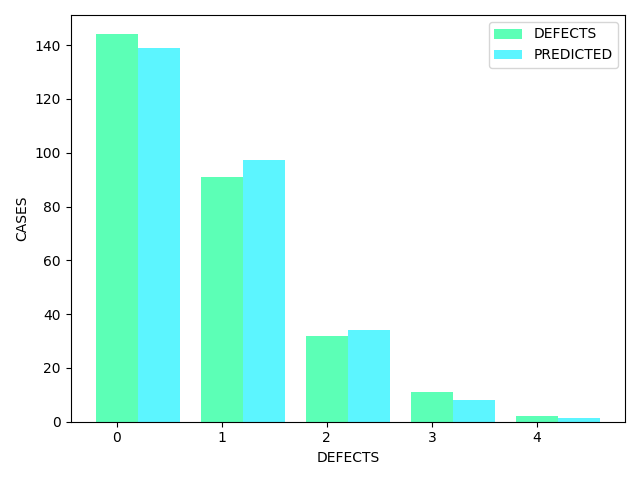
\includegraphics[width=\textwidth,height=\textheight,keepaspectratio]{Figure_1.png}
	
	\subproblem{e} According to the barplot in (c), does the poisson distribution fit the data well? Compare the values of the actual cases and the values of the poisson predicted cases, and write your opinions about performance of the distribution.\\
	As we can see in the table the real and predicted values  are close to each other. We can say that the distribution data almost fit.
	So we can make close predictions using poisson distribution.
	
	\subproblem{f} According to your estimations above, write your opinions considering your barplot and Table \ref{tab2}.Do you think that road transportation is dangerous for us? Whether yes or no, explain your reason.\\
	There is not defects half of them but still we can not ignore the other half so we can not say its not dangerous. since the predicted values almost satisfy the real ones.
	
	\subproblem{g} Paste your code that you implemented for the subproblems above. Do not forget to write comments on your code.\\
	Example:\\
	\begin{itemize}
		\item The common code block for all subproblems\\
		Paste here. Your code should read the file and compute other things which the following subproblems need.
		\item The code block for (a)\\
		\item{
		  \begin{lstlisting}
from numpy import printoptions
import matplotlib.pyplot as plt
import math
import pandas as pd
nl_count=0
#count line number
file = open("manufacturing_defects.txt", "r")
for line in file:
    if line != "\n":
        nl_count += 1
file.close()
#count column number
tab_count=0
for ch in line:
    if ch == "\t":
        tab_count+=1
#creating a dictionary and add the defects number for different number defects
total_each = dict()
file = open("manufacturing_defects.txt", "r")
for line in file:
    value = line.split('\t')
    for i in value[2:]:
        index = int(i)
        if index in total_each:
            total_each[index]+=1
        else:
            total_each[index] =1
file.close()
print("Give a table how many cases occur for all companies between 2000 and 2019 for each number of defects")
#printing table
print("# of Defects |# of cases in all company between the years")
print("---------------------------------------------------------")
for i in range(0, len(total_each)):
    print(str(i),"           |",str(total_each[i]))
		  \end{lstlisting}
		  }
		Paste here. Your code should compute the values in Table \ref{tab1} column 2.
		\item The code block for (b)\\
		\item{
		  \begin{lstlisting}
print(" Estimate λ from the given data.")
total1=0
total2=0
#calculating lamda as indicated part b
for i in range(0, len(total_each)):
    total1+= total_each[i]*i
for i in range(0, len(total_each)):
    total2+= total_each[i]
print(total1/total2)
lamda=total1/total2

		  \end{lstlisting}
		  }
		Paste here. Your code should compute $\lambda$.
		\item The code block for (c)\\
		\item{
		  \begin{lstlisting}
#collecting predicted values in another dictionary
each_predict= dict()
print("Update Table 1 in Table 2 with Poisson predicted cases with the estimated λ.")
#Poisson formula for each one
for i in range(0, len(total_each)):
    each_predict[i] =  pow(math.e, -1*lamda)* pow(lamda, i)
    each_predict[i]/= math.factorial(i)
    each_predict[i]*= total2

print("# of Defects |# of cases in all company between the years|")
print("---------------------------------------------------------")
for i in range(0, len(total_each)):
    print(str(i),"           |",str(total_each[i]),"       |",each_predict[i])
		  \end{lstlisting}
		  }
		Paste here. Your code should compute the values in Table \ref{tab2} column 3. 
		\item The code block for (d)\\
		\item{
		  \begin{lstlisting}
print("Update Table 1 in Table 2 with Poisson predicted cases with the estimated λ.")
#creating values from list of predicted and actual values
total_each_l= []
each_predict_l = []
for i in total_each:
    total_each_l.append(total_each[i])
    each_predict_l.append(each_predict[i])

defects_var = []
for i in total_each:
    defects_var.append(i)

size = len(total_each)
arangee = numpy.arange(size)
opacity = 0.8
#graph x and y values
pltx = plt.bar(arangee,total_each_l, 0.40, alpha=opacity, color='#33FFA4', label='DEFECTS')
plty = plt.bar(arangee+0.40, each_predict_l, 0.40, alpha=opacity,color='#33F3FF', label='PREDICTED')
#graph labels
plt.xlabel('DEFECTS')
plt.ylabel('CASES')
plt.xticks(arangee)
plt.legend()

plt.tight_layout()
plt.show()


		  \end{lstlisting}
		  }
		Paste here. Your code should draw the barplot.
	\end{itemize}
	
	
	
	
\end{document} 


